%!TEX root = ../TI_Gomez_Luis.tex
\chapter{Diseño e implementación} % Main chapter title

\label{Chapter3} % Change X to a consecutive number; for referencing this chapter elsewhere, use \ref{ChapterX}

\definecolor{mygreen}{rgb}{0,0.6,0}
\definecolor{mygray}{rgb}{0.5,0.5,0.5}
\definecolor{mymauve}{rgb}{0.58,0,0.82}

%%%%%%%%%%%%%%%%%%%%%%%%%%%%%%%%%%%%%%%%%%%%%%%%%%%%%%%%%%%%%%%%%%%%%%%%%%%%%
% parámetros para configurar el formato del código en los entornos lstlisting
%%%%%%%%%%%%%%%%%%%%%%%%%%%%%%%%%%%%%%%%%%%%%%%%%%%%%%%%%%%%%%%%%%%%%%%%%%%%%
\lstset{ %
  backgroundcolor=\color{white},   % choose the background color; you must add \usepackage{color} or \usepackage{xcolor}
  basicstyle=\footnotesize,        % the size of the fonts that are used for the code
  breakatwhitespace=false,         % sets if automatic breaks should only happen at whitespace
  breaklines=true,                 % sets automatic line breaking
  captionpos=b,                    % sets the caption-position to bottom
  commentstyle=\color{mygreen},    % comment style
  deletekeywords={...},            % if you want to delete keywords from the given language
  %escapeinside={\%*}{*)},          % if you want to add LaTeX within your code
  %extendedchars=true,              % lets you use non-ASCII characters; for 8-bits encodings only, does not work with UTF-8
  %frame=single,	                % adds a frame around the code
  keepspaces=true,                 % keeps spaces in text, useful for keeping indentation of code (possibly needs columns=flexible)
  keywordstyle=\color{blue},       % keyword style
  language=[ANSI]C,                % the language of the code
  %otherkeywords={*,...},           % if you want to add more keywords to the set
  numbers=left,                    % where to put the line-numbers; possible values are (none, left, right)
  numbersep=5pt,                   % how far the line-numbers are from the code
  numberstyle=\tiny\color{mygray}, % the style that is used for the line-numbers
  rulecolor=\color{black},         % if not set, the frame-color may be changed on line-breaks within not-black text (e.g. comments (green here))
  showspaces=false,                % show spaces everywhere adding particular underscores; it overrides 'showstringspaces'
  showstringspaces=false,          % underline spaces within strings only
  showtabs=false,                  % show tabs within strings adding particular underscores
  stepnumber=1,                    % the step between two line-numbers. If it's 1, each line will be numbered
  stringstyle=\color{mymauve},     % string literal style
  tabsize=2,	                   % sets default tabsize to 2 spaces
  title=\lstname,                  % show the filename of files included with \lstinputlisting; also try caption instead of title
  morecomment=[s]{/*}{*/}
}


%----------------------------------------------------------------------------------------
%	SECTION 1
%----------------------------------------------------------------------------------------


Este capítulo presenta el diseño e implementación del sistema de medición de \MPF. La arquitectura desarrollada integró componentes de hardware y software para cumplir los requerimientos técnicos establecidos. El diseño incorporó cinco subsistemas principales: adquisición de datos mediante sensores redundantes, sistema de alimentación con respaldo, unidad de procesamiento basada en microcontrolador, almacenamiento local de datos y comunicación inalámbrica.

La implementación siguió un enfoque modular que permitió el desarrollo incremental y la verificación independiente de cada componente. El sistema integró múltiples protocolos de comunicación para la interacción entre módulos, mientras que la arquitectura de software estableció capas de abstracción para facilitar la mantenibilidad y escalabilidad del sistema.

%Las siguientes secciones detallan los requerimientos técnicos, la selección de componentes, el diseño de hardware, la arquitectura de software y los procedimientos de calibración implementados.




\section{Arquitectura general del sistema}
%	1	Descripción general de cada uno de los componentes de Hardware empleado	Imagen con los componetes principales	Lista de componentes y sus funciones

La implementación del monitor de \MPF requirió un conjunto específico de componentes de hardware para cumplir los requerimientos técnicos establecidos. La arquitectura del sistema se estructuró en cuatro subsistemas principales:
\begin{itemize}
	\item Sistema de alimentación con la fuente S-25-5.
	\item Unidad de procesamiento basada en el microcontrolador STM32F429.
	\item Módulos de medición con tres sensores SPS30, un RTC y un sensor DHT22.
	\item Sistema de almacenamiento y comunicación con módulo microSD y ESP8266.
\end{itemize}

La figura \ref{fig:diagBloques2} presenta el diagrama de bloques de la arquitectura. Las especificaciones técnicas de cada componente se detallan en las siguientes subsecciones.

\begin{figure}[h]
	\center
	%!TEX root = ../TI_Gomez_Luis.tex
	\centering
	\shorthandoff{<>} % Desactivar caracteres problemáticos
%	\begin{tikzpicture}[ node distance=1.5cm]
%	% Nodes
%	\node (microcontroller) 
%	[draw, rectangle, fill=blue!10!white, align=center] 						
%	{\textbf{Microcontrolador}\\ \rotatebox{90}{\faMicrochip}};  
%	
%	\node (sensor1) 		
%	[above right=of microcontroller, draw, rectangle, fill=red!10!white, align=center, yshift=0.2cm, xshift=0.3cm] 	
%	{Sensor de\\MP2,5 \faSmog};
%	
%	\node (sensor2) 		
%	[right=of microcontroller, draw, rectangle, fill=red!10!white, align=center] 		
%	{Sensor de\\MP2,5 \faSmog};
%	
%	\node (sensor3) 		
%	[below right=of microcontroller, draw, rectangle, fill=red!10!white, align=center, , yshift=-0.2cm, xshift=0.3cm] 	
%	{Sensor de\\MP2,5 \faSmog};
%	
%	\node (storage) 		
%	[below=of microcontroller, draw, fill=yellow!10!white, rectangle, align=center] 		
%	{Sistema de \\ almacenamiento  \faSdCard }; % \faDatabase
%	
%	\node (transmission) 	
%	[above=of microcontroller, draw, rectangle, align=center] 		
%	{Sistema de transmi-\\sión de datos  \faSignal};
%	
%	\node (rtc) 			
%	[above left=of microcontroller, draw, rectangle, align=center, yshift=-1.5cm, xshift=-.33cm]  
%	{RTC \faClock[regular]};
%	
%	\node (power) 			
%	[below left=of microcontroller, draw, rectangle, align=center,yshift=-0.2cm, xshift=0.0cm] 	
%	{Fuente de\\poder \faBatteryQuarter};
%	
%	\node (cabinet) 		[above right=of transmission,  xshift=-6.8cm,yshift=-0.7cm]     {\textbf{Gabinete} \faCloudSunRain};
%	
%	% Bounding Box
%	\begin{scope}[on background layer]
%	\node[fill=gray!10,  draw, rectangle, rounded corners, fit=(cabinet) (sensor2) (rtc) (storage) (transmission)] {};
%	\end{scope}
%	
%	% Arrows
%	\draw[<->] (microcontroller) -- (sensor1);
%	\draw[<->] (microcontroller) -- (sensor2);
%	\draw[<->] (microcontroller) -- (sensor3);
%	\draw[<->] (microcontroller) -- (storage);
%	\draw[<->] (microcontroller) -- (transmission);
%	\draw[->] (rtc) -- (microcontroller);
%	\draw[->] (power) -- (microcontroller);
%	\end{tikzpicture}
	 % Reactivar caracteres problemáticos

	
	\begin{tikzpicture}[
	node distance=2.5cm,
	box/.style={
		draw,
		rectangle,
		minimum width=2.5cm,
		minimum height=1.2cm,
		align=center,
		rounded corners=2pt,
		fill=white,
		font=\small
	},
	subsystem/.style={
		draw,
		thick,
		rounded corners=4pt,
		fill=gray!10,
		inner sep=0.5cm,
		inner ysep=0.8cm,
		minimum width=3cm
	},
	label/.style={
		font=\bfseries,
		text=black,
		anchor=south,
		align=center
	}
	]
	
	% Sistema de Adquisición de Datos
	\begin{scope}[local bounding box=sensors]
	\coordinate (sensor_origin) at (0.2,2.7);
	\node[subsystem, minimum width=3cm, minimum height=8cm] (sensor_group) at (sensor_origin) {};
	\node[label] at ($(sensor_group.north)+(0,-1.3)$) {sistema de\\ adquisición};
	
	% Componentes del subsistema de adquisición
	\node[box, minimum width=2cm] (s1) at ($(sensor_origin)+(0,2.1)$) {sensor \#1 \\  \MPF \faSmog};
	\node[box, minimum width=2cm] (s2) at ($(sensor_origin)+(0,0.8)$) {sensor \#2 \\  \MPF \faSmog};
	\node[box, minimum width=2cm] (s3) at ($(sensor_origin)+(0,-0.5)$) {sensor \#3 \\  \MPF \faSmog};
	\node[box, minimum width=2cm] (dht) at ($(sensor_origin)+(0,-1.8)$) {DHT22\\ \faThermometerHalf };
	\node[box, minimum width=2cm] (rtc) at ($(sensor_origin)+(0,-3.3)$) {RTC  \faClock[regular]\\ DS3231};
	\end{scope}
	
	% Unidad de Procesamiento
	\begin{scope}[local bounding box=processing]
	\coordinate (proc_origin) at (4.5,4);
	\node[subsystem, minimum width=5cm, minimum height=4.7cm] (proc_group) at (proc_origin) {};
	\node[label] at ($(proc_group.north)+(0,-1.1)$) {unidad de\\ procesamiento};
	
	\node[box, minimum width=3.5cm, minimum height=2.5cm] (mcu) at ($(sensor_origin)+(4.3,0.7)$) {microcontrolador\\STM32F429\\\rotatebox{90}{\faMicrochip}};
	\end{scope}
	
	% Sistema de Almacenamiento y Comunicación
	\begin{scope}[local bounding box=storage]
	\coordinate (storage_origin) at (9,4);
	\node[subsystem, minimum width=3.5cm, minimum height=4.7cm] (storage_group) at (storage_origin) {};
	\node[label] at ($(storage_group.north)+(0,-1.2)$) {almacenamiento\\ y comunicación};
	
	\node[box] (sd) at ($(storage_origin)+(0,0.5)$) {microSD\\ \faSdCard };
	\node[box] (wifi) at ($(storage_origin)+(0,-1.2)$) {módulo Wi-Fi\\ \faSignal};
	\end{scope}
	
	% Sistema de Alimentación
	\begin{scope}[local bounding box=power]
	\coordinate (power_origin) at (4.5,0);
	\node[subsystem, minimum width=5cm, minimum height=2.5cm] (power_group) at (power_origin) {};
	\node[label] at ($(power_group.north)+(0,-2.5)$) {sistema de alimentación};
	
	\node[box,  minimum width=1.8cm, minimum height=1cm] (ps) at ($(power_origin)+(-1,0)$) {Fuente\\ Principal\\ \faChargingStation};
	\node[box,  minimum width=1.8cm, minimum height=1cm] (bat) at ($(power_origin)+(1,0)$) {batería\\ backup\\ \faBatteryQuarter};
	\end{scope}
	
	% Sistema de Control y Monitoreo
	\begin{scope}[local bounding box=monitoring]
	\coordinate (monitor_origin) at (9,0);
	\node[subsystem, minimum width=3.5cm, minimum height=2.5cm] (monitor_group) at (monitor_origin) {};
	\node[label] at ($(monitor_group.north)+(0,-2.4)$) {control y\\ monitoreo};
	
	\node[box, minimum width=2cm] (led) at ($(monitor_group.north)+(0,-0.8)$){\faLightbulb[regular] LED\\ estado};
	\end{scope}
	
	% Conexiones entre los componentes
	\foreach \i in {s1,s2,s3,dht,rtc}
	\draw[->, thick] (\i) -- (mcu);
	
	\draw[<->, thick] (mcu) -- (sd);
	\draw[<->, thick] (mcu) -- (wifi);
	\draw[->, thick] (ps) -- (mcu);
	\draw[->, thick, dashed] (bat) -- (mcu);
	\draw[->, thick] (mcu) -- (led);
	
	% Gabinete exterior (envolviendo todos los subsistemas)
	\begin{scope}[on background layer]
	\node[draw, thick, rounded corners=6pt, fill=gray!5, 
	fit=(sensors) (processing) (storage) (power) (monitoring),
	inner sep=0.5cm] (cabinet) {};
	\end{scope}
	
	% Título del gabinete exterior
	\node[label] at ($(cabinet.north)+(-0.5,-.8)$) {Gabinete IP65  \faCloudSunRain};
	\end{tikzpicture}
	\shorthandon{<>}

	\caption{Esquema de bloques del instrumento de \MPF.}
	\label{fig:diagBloques2}
\end{figure}

\pagebreak

%2	Aspectos generales del diseño y la implementación	Diagrama general del sistema	-
\section{Selección y diseño de hardware}	
%2	Justificación de la selección de componentes	Gráficos comparativos de componentes	Matriz de decisión de componentes


La selección de componentes para el sistema de medición de \MPF se realizó mediante un análisis de las alternativas disponibles en el mercado, lo que consideró factores técnicos, económicos y de disponibilidad. Se empleó una matriz de decisión ponderada para evaluar cada componente crítico del sistema.

\subsection{Sensor de material particulado}

La selección del sensor SPS30 se fundamentó en un análisis comparativo con otros sensores disponibles en el mercado, como se muestra en la tabla \ref{tab:comparacion_sensores}.

\begin{table}[htbp]
	\centering
	\small
	\caption{Comparación de sensores de material particulado}
	\label{tab:comparacion_sensores}
% comparacion de sensores de MP
	\begin{tabular}{lcccc}
		\toprule
		\textbf{Característica} & \textbf{SPS30} & \textbf{PMS5003} & \textbf{SDS011} & \textbf{GP2Y1010AU0F} \\
		\midrule
		Precisión (\%) & $\pm$10 & $\pm$15 & $\pm$15 & $\pm$25 \\
		Rango (\SI{}{\micro\gram\per\cubic\meter}) & 0-1000 & 0-500 & 0-999 & 0-500 \\
		Interfaces & \IIC/UART & UART & UART & Analógico \\
		Vida útil (h) & >\num{20000} & >\num{8000} & >\num{8000} & >\num{5000} \\
		Auto-limpieza & Sí & No & No & No \\
		Costo relativo & 1,5x & 1,0x & 1,2x & 0,5x \\
		\bottomrule
	\end{tabular}
\end{table}

El SPS30 destaca por su precisión y sistema de auto-limpieza, características cruciales para mediciones a largo plazo. La interfaz \IIC y UART facilita la integración con el microcontrolador seleccionado.

\newpage
\subsection{Microcontrolador}

La elección del STM32F429ZI se basó en los siguientes criterios ponderados, como se detalla en la tabla \ref{tab:decision_micro}.

\begin{table}[htbp]
	\centering
	\small
	\caption{Matriz de decisión para selección del microcontrolador.}
	\label{tab:decision_micro}
% comparacion microcontrolador
	\begin{tabular}{lccccc}
		\toprule
		\textbf{Criterio} & \textbf{Peso} & \textbf{STM32F429} & \textbf{ESP32} & \textbf{RP2040} & \textbf{SAMD21} \\
		\midrule
		Velocidad CPU & 0,25 & 5 (1,25) & 4 (1,00) & 3 (0,75) & 3 (0,75) \\
		Memoria & 0,20 & 5 (1,00) & 4 (0,80) & 3 (0,60) & 2 (0,40) \\
		Periféricos & 0,20 & 5 (1,00) & 4 (0,80) & 3 (0,60) & 3 (0,60) \\
		FPU & 0,15 & 5 (0,75) & 5 (0,75) & 2 (0,30) & 2 (0,30) \\
		Documentación & 0,10 & 5 (0,50) & 4 (0,40) & 3 (0,30) & 3 (0,30) \\
		Costo & 0,10 & 3 (0,30) & 4 (0,40) & 5 (0,50) & 4 (0,40) \\
		\midrule
		\textbf{Total} & 1,00 & \textbf{4,80} & 4,15 & 3,05 & 2,75 \\
		\bottomrule
	\end{tabular}
	\caption*{Nota: Los valores en paréntesis representan la puntuación ponderada (criterio × peso)}
\end{table}

\subsection{Módulos de comunicación y almacenamiento}

Para el sistema de comunicación inalámbrica, se seleccionó el módulo ESP8266 por su balance entre costo, consumo energético y facilidad de implementación. La tabla \ref{tab:modulos_comunicacion} presenta la comparativa de alternativas evaluadas.

\begin{table}[htbp]
	\centering
	\small
	\caption{Comparación de módulos de comunicación inalámbrica.}
	\label{tab:modulos_comunicacion}
	
% comparacion modulo comunicacion
\begin{tabular}{lcccc}
	\toprule
	\textbf{Característica} & \textbf{ESP8266} & \textbf{nRF24L01} & \textbf{HC-12} & \textbf{RN4870} \\
	\midrule
	Protocolo & Wi-Fi & RF \SI{2,4}{\giga\hertz} & RF \SI{433}{\mega\hertz} & BLE \\
	Alcance (\si{\meter}) & \num{100}+ & \num{100} & \num{1000} & \num{50} \\
	Velocidad (\si{\mega\bit\per\second}) & \num{72,2} & \num{2} & \num{0,01} & \num{1} \\
	Consumo (\si{\milli\ampere}) & \num{80} & \num{15} & \num{100} & \num{10} \\
	Costo relativo & \num{1,0}x & \num{0,5}x & \num{2,0}x & \num{3,0}x \\
	\bottomrule
\end{tabular}
\end{table}

\subsection{Componentes de soporte}

Los componentes adicionales como el RTC DS3231 y el módulo microSD se priorizó la confiabilidad y compatibilidad con el sistema. El DS3231, en comparación con DS1707, destaca por su precisión temporal de \SI{\pm2}{\ppm} y compensación de temperatura integrada. Para el almacenamiento, el módulo microSD ofrece capacidad escalable y compatibilidad con el sistema de archivos FAT32, lo que facilita el acceso a los datos almacenados. La memoria extraíble permitió la recuperación y transferencia de datos a otros dispositivos para su análisis posterior.


\section{Esquemático y PCB}	
%2	Detalles del diseño electrónico	Esquemático del circuito, Diseño de PCB	Listado de materiales (BOM)

El diseño electrónico del instrumento de medición de \MPF integró cinco subsistemas interconectados. En la figura \ref{fig:esquematicogeneral} se observa el esquemático general del sistema, que incorporó los bloques funcionales principales: procesamiento central, sensores redundantes, sistema de almacenamiento, comunicación inalámbrica y alimentación.

% TODO: \usepackage{graphicx} required
\begin{figure}[H]
	\centering
	\includegraphics[width=1\linewidth]{Figures/esquema_general}
	\caption{Esquema general del instrumento de \MPF con su respectivas conexiones da datos.}
	\label{fig:esquematicogeneral}
\end{figure}

La unidad de procesamiento se implementó mediante el microcontrolador STM32 Nucleo F429ZI, que estableció las interfaces de comunicación con los periféricos a través de los protocolos UART, SPI e \IIC. El diseño incluyó tres sensores SPS30 conectados mediante UART para la medición redundante de \MPF. Esta configuración permitió la validación cruzada de datos y mejoró la confiabilidad del sistema.

El subsistema de almacenamiento y comunicación integró un socket para tarjeta microSD mediante interfaz SPI y el módulo ESP8266 para transmisión inalámbrica vía UART. La gestión temporal se implementó con el RTC DS3231 conectado mediante \IIC. El sistema de alimentación incorporó la fuente S-25-5 con protección contra sobretensiones y un circuito de respaldo mediante batería.

La figura \ref{fig:pcbtesismp} muestra el diseño de la placa de circuito impreso (PCB) de cuatro capas. La disposición de componentes priorizó la separación física entre las secciones analógica y digital para minimizar interferencias electromagnéticas. El ruteo implementó las siguientes consideraciones de diseño:

\begin{itemize}
	\item Plano de tierra dedicado en la capa interna para reducir interferencias.
	\item Pistas de alimentación dimensionadas para corrientes máximas de \SI{2}{\ampere}.
	\item Vías térmicas para disipación en reguladores de tensión.
	\item Filtros LC en las líneas de alimentación de sensores.
	\item Conectores con retención mecánica para mayor confiabilidad.
\end{itemize}



% TODO: \usepackage{graphicx} required
\begin{figure}[H]
	\centering
	\includegraphics[width=1\linewidth]{Figures/PCB_Tesis_MP}
	\caption{PCB del instrumento de \MPF.}
	\label{fig:pcbtesismp}
\end{figure}


La tabla \ref{tab:bom} presenta la lista de materiales (BOM) con los componentes principales del sistema.

\begin{table}[!hbp]
	\centering
	\caption{Lista de materiales principales del instrumento}
	\label{tab:bom}
	\small
	\begin{tabular}{llcc}
		\toprule
		\textbf{Componente} & \textbf{Descripción} & \textbf{Cantidad} & \textbf{Referencia} \\
		\midrule
		STM32F429ZI & Microcontrolador & 1 & U7 \\
		SPS30 & Sensor MP2.5 & 3 & U4,U5,U6 \\
		DS3231 & RTC & 1 & U8 \\
		ESP8266 & Módulo WiFi & 1 & U7 \\
		S-25-5 & Fuente 5V & 1 & PS1 \\
		\bottomrule
	\end{tabular}
\end{table}


El diseño final resultó en una PCB de \SI{150x120}{\milli\meter} con montaje mixto de componentes THT y SMD. La disposición facilitó el acceso para mantenimiento y permitió la instalación en gabinetes industriales estándar.

El diseño de la placa de circuito impreso (PCB) se realizó conforme a un conjunto de reglas y restricciones técnicas que aseguraron su fabricación adecuada. La tabla \ref{tab:reglas_pcb} presenta los parámetros mínimos establecidos para la fabricación, organizados en cuatro categorías principales: especificaciones de cobre, orificios, vías enterradas y serigrafía. Estos valores se ajustaron a las capacidades estándar de los fabricantes de PCB y permitieron mantener la integridad de las señales mientras se optimizó el espacio disponible.

Complementariamente, la tabla \ref{tab:clases_redes} muestra las tres clases de redes implementadas en el diseño, cada una con configuraciones específicas según sus requisitos funcionales. La clase "Default" se aplicó a señales de propósito general, mientras que la clase "microSD" implementó márgenes más reducidos (0,15 mm) para las conexiones del módulo de almacenamiento, lo que facilitó el ruteo en áreas de alta densidad. Por otro lado, la clase "potencia" incorporó pistas más anchas (0,5 mm) y vías de mayor diámetro (0,8 mm) para soportar las corrientes requeridas por los componentes del sistema sin generar caídas de tensión significativas o sobrecalentamiento.

\section{Arquitectura de software}

La arquitectura de software del sistema de medición de \MPF se implementó mediante una estructura modular que aseguró la funcionalidad, mantenibilidad y escalabilidad del sistema. El diseño incorporó cuatro patrones arquitectónicos.

\subsection{Patrones arquitectónicos fundamentales}

La implementación adoptó una arquitectura en capas, como se muestra en la figura \ref{fig:patroncapas}. El software se organizó en tres niveles de abstracción principales. La capa de aplicación contiene los procesos principales del sistema, incluyendo la adquisición de datos, procesamiento estadístico y gestión de comunicaciones. La capa de drivers implementó los controladores específicos para cada dispositivo periférico, mientras que la capa HAL (\textit{Hardware Abstraction Layer}) proporcionó una interfaz estandarizada para el acceso al hardware. Esta estructura en capas facilitó la portabilidad del código y permitió el desarrollo independiente de cada nivel de abstracción.

\begin{figure} [H]
	\centering
	\small
	%\includegraphics[width=0.2\linewidth]{Figures/PatronCapas}
	%patron de capas
	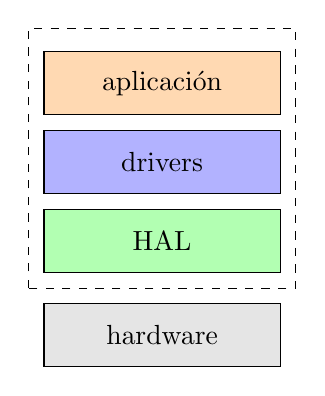
\begin{tikzpicture}
	% Define separated layers
	\node[draw, fill=orange!30, minimum width=3cm, minimum height=0.8cm] at (0, 2) {aplicación};
	\node[draw, fill=blue!30, minimum width=3cm, minimum height=0.8cm] at (0, 1.0) {drivers};
	\node[draw, fill=green!30, minimum width=3cm, minimum height=0.8cm] at (0, 0) {HAL};
	\node[draw, fill=gray!20, minimum width=3cm, minimum height=0.8cm] at (0, -1.2) {hardware};
	
	% Outline dashed box surrounding only the top three layers
	\draw[dashed] (-1.7, -0.6) rectangle (1.7, 2.7);
	\end{tikzpicture}
	\caption{Patrón de arquitectura de capas, obtenido a partir de presentaciones de clases de Ingeniería de Software \protect\footnotemark.}
	\label{fig:patroncapas}
\end{figure}
\footnotetext{Imagen obtenida de diapositiva de la materia Ingeniería de Software,  CESE, FIUBA, 2023.}

El patrón ``observar y reaccionar'', que se muestra en la figura \ref{fig:patronobservarreaccionar}, es la base del sistema de monitoreo. Su implementación en la capa de aplicación permitió la supervisión continua de los sensores y el procesamiento sistemático de los datos. El diseño implementó un mecanismo de notificación basado en el patrón de observador, donde los sensores funcionaron como sujetos observables, lo que generó eventos o cambios de estado. Por otro lado, los módulos de procesamiento y almacenamiento fueron diseñados como observadores, encargados de recibir y procesar las notificaciones emitidas por los sujetos observables.

\begin{figure}[H]
	\footnotesize
	\centering
	% Patron Obervar y reaccionar
	

\shorthandoff{>}
\begin{tikzpicture}[
node distance=0.5cm,
every node/.style={
	draw,
	rounded corners,
	minimum height=1cm,
	minimum width=2.5cm,
	align=center 
},
label/.style={    % Nuevo estilo para etiquetas
	draw=none,    % Sin borde
	minimum height=0cm,  % Sin altura mínima
	minimum width=0cm   % Sin ancho mínimo
}
]
% Definición de nodos
\node (observer) {proceso\\ observador};
\node[above=0.5cm of observer] (sensors) {sensores};
\node[right=2cm of observer] (analysis) {proceso de\\ análisis};
\node[right=2cm of analysis] (display) {proceso de\\ despliegue};
\node[above=0.5cm of display] (screen) {pantalla};
\node[below left=0.5cm and 0.5cm of analysis] (alarm) {proceso de\\ alarma};
\node[below right=0.5cm and 1cm of analysis] (reactor) {proceso reactor};
\node[below=of alarm] (alarmDevice) {alarma};
\node[below=of reactor] (otherDevice) {otro equipo};

% Conexiones
\draw[-latex] (sensors) -- (observer);
\draw[-latex] (observer) -- node[label, above] {valores de\\ sensor} (analysis);
\draw[-latex] (analysis) -- node[label, above] {valores a\\ desplegar} (display);
\draw[-latex] (display) -- (screen);
\draw[-latex] (analysis) -- (alarm);
\draw[-latex] (alarm) -- (alarmDevice);
\draw[-latex] (analysis) -- (reactor);
\draw[-latex] (reactor) -- (otherDevice);
\end{tikzpicture}
\shorthandon{>}
	\caption{Patrón arquitectónico: ``observar y reaccionar'' \protect\footnotemark.}
	\label{fig:patronobservarreaccionar}
\end{figure}
\footnotetext{Imagen obtenida de diapositiva de la materia Ingeniería de Software,  CESE, FIUBA, 2023.}

El tercer patrón implementado, ``segmentación de procesos'', estableció el flujo de datos entre los módulos del sistema. Un esquema de este patrón puede ser observado en la figura \ref{fig:patronsegmentacionprocesos}. Esta arquitectura definió etapas específicas para la adquisición, validación, procesamiento estadístico y almacenamiento de las mediciones. La segmentación aseguró la integridad de los datos mediante buffers intermedios entre etapas y mecanismos de verificación en cada transferencia. Esta implementación permitió el procesamiento secuencial de las mediciones y facilitó la detección de errores en el flujo de datos.

\begin{figure}[H]
	\centering
	\small
	% patron de segmentacion
		\shorthandoff{>}
		\begin{tikzpicture}[node distance=5cm, every node/.style={draw, rounded corners, minimum height=1.5cm, minimum width=2.2cm, align=center}]
			% Nodes
			\node (producer) {proceso\\ productor};
			\node[right of=producer] (buffer) {proceso\\ buffer};
			\node[right of=buffer] (consumer) {proceso\\ consumidor};
			\node[right=1cm of consumer, draw=none, minimum width=0.1cm] (ellipsis) {...};
			
			% Connections with labels outside of boxes
			\path[-latex] (producer) edge node[above, draw=none] {datos\\ producidos} (buffer);
			\path[-latex] (buffer) edge node[above, draw=none] {datos\\ consumidos} (consumer);
			\path[-latex] (consumer) edge (ellipsis);
		\end{tikzpicture}
		\shorthandon{>}
	\caption{ Patrón arquitectónico: “segmentación de procesos” \protect\footnotemark.}
	\label{fig:patronsegmentacionprocesos}
\end{figure}
\footnotetext{Imagen obtenida de diapositiva de la materia Ingeniería de Software,  CESE, FIUBA, 2023.}


\subsection{Integración de las estructuras y flujo de datos}

La figura \ref{fig:diagpatrones} presenta la integración de la arquitectura de software del sistema. La implementación estableció procesos interconectados para la gestión del flujo de datos, desde la adquisición en los sensores hasta el almacenamiento y transmisión de la información. Estos procesos incluyeron la validación de mediciones, el procesamiento estadístico, el almacenamiento local y la comunicación con sistemas remotos.

\begin{figure}[htpb]
	\centering
	\footnotesize
		
	\shorthandoff{<>} % Desactivar caracteres problemáticos
	
	
	\begin{tikzpicture}[ node distance=1cm]
	% Nodes
	%\draw[rounded corners] (0,0) rectangle (4,2);
	
	\node (observador) 
	[draw, rectangle, rounded corners, fill=blue!10!white, 
	align=center, yshift=2cm, xshift=0cm] 						
	{proceso\\ observador}; %\rotatebox{90}{\faMicrochip}};  
	
	\node (sensor1) 		
	[above left=of observador, draw, circle, fill=red!10!white, align=center, yshift=0.1cm, xshift=1cm] 	
	{\faSmog};
	
	\node (sensor2) 		
	[above=of observador, draw, circle, fill=red!10!white, align=center, yshift=-0.3cm, xshift=0.0cm] 	
	{ \faSmog};
	
	\node (sensor3)
	[above right=of observador, draw, circle, fill=red!10!white, align=center, yshift=0.1cm, xshift=-.80cm]
	{\faSmog};
	
	\node (rtc) 			
	[below =of observador, draw, circle, align=center,fill=red!10!white, yshift=0cm, xshift=0.0cm]  
	{\faClock[regular]};
	\node (sensorRTC) [below=of rtc,align=center, xshift=0 cm,yshift=1cm]     {\textbf{RTC} }; %\faCloudSunRain
	
	
	\node (tyh) 			
	[below  right=of observador, draw, circle, align=center,fill=red!10!white, yshift=0cm, xshift=-1.0cm]  {\faThermometerHalf};
	\node (sensorTyH) [below=of tyh, align=center, xshift=0.1 cm,yshift=1cm] 
	{\textbf{TyH} }; %\faCloudSunRain


	
	\node (sensores) [above =of sensor1,align=center, xshift=1 cm,yshift=-1cm]     {\textbf{sensores  \MPF} }; %\faCloudSunRain
	
	\node (aplicacion) 
	[right=2cm of sensores,align=center, xshift=-0.5 cm,yshift=0.2cm]     
	{\textbf{capa aplicación} }; %\faCloudSunRain
	
	\node (segmentacion) 		
	[right=of observador, draw, rectangle, rounded corners, fill=red!30!white, align=center, yshift=0cm, xshift=0cm] 						
	{ patrón \\ segmentación}	;
	
	\node (analisis) 		
	[right=of segmentacion, draw, rectangle, rounded corners, fill=blue!10!white, align=center, yshift=0cm, xshift=0cm] 						
	{proceso \\ de análisis};
	
	\node (despliegue) 		
	[right=of analisis, draw, rectangle, rounded corners, fill=blue!10!white, align=center, yshift=0cm, xshift=0cm] 						
	{proceso \\ despliegue};
	
	\node (alarma)
	[below left=of analisis, draw, rectangle, rounded corners, fill=blue!10!white, align=center, yshift=0cm, xshift=1cm] 						
	{proceso \\ alarma};
	
	\node (reactor) 		
	[below right=of analisis, draw, rectangle, rounded corners, fill=blue!10!white, 	align=center, yshift=0cm, xshift=0cm] 						
	{ proceso \\ reactor};
	
	\node (servidor) 		
	[below=0.4 cm of reactor,  align=center, yshift=0cm, xshift=0cm] 						
	{módulo\\inalámbrico \faWifi}; % https://www.ipgp.fr/~moguilny/LaTeX/fontawesome5Icons.pdf
	
	\node (led) 		
	[below=0.5cm of alarma,  align=center, yshift=0cm, xshift=0cm] 						
	{LED \faLightbulb};
	
	\node (memoria) 		
	[above=of despliegue,  align=center, yshift=0cm, xshift=0cm] 						
	{memoria \faSdCard };
	
	% Bounding Box
	\begin{scope}[on background layer]
	\node(aplicacion)[fill=orange!15,  draw, rectangle, rounded corners, fit=(aplicacion)(sensor1) (sensor2) (sensor3) (sensores) (despliegue) (rtc) (servidor) (alarma)] {};
	\node(driver)[below=of aplicacion,fill=blue!15,  draw, rectangle, rounded corners,
	minimum width=11cm, minimum height=0.8cm, , yshift=0.8cm, xshift=0cm]{capa drivers} ;
	\node(hal)[below=of driver,fill=green!10,  draw, rectangle, rounded corners,
	minimum width=11cm, minimum height=0.8cm, yshift=0.8cm]{capa HAL} ;
	\node(hardware)[below=of hal,fill=gray!10,  draw, rectangle, rounded corners,
	minimum width=11cm, minimum height=0.8cm,  yshift=0.5cm]{Hardware} ;
	\node[draw, dashed, fit=(aplicacion) (driver) (hal), inner sep=8pt, rounded corners] (box) {};
	\end{scope}
	
	% Arrows
	\draw[-] (observador) -- (sensor1);
	\draw[-] (observador) -- (sensor2);
	\draw[-] (observador) -- (sensor3);
	\draw[->] (observador) -- (segmentacion);
	\draw[->] (segmentacion) -- (analisis);
	\draw[->] (analisis) -- (despliegue);
	\draw[->] (despliegue) -- (memoria);
	\draw[->] (analisis) -- (reactor);
	\draw[->] (reactor) -- (servidor); % \faWifi
	\draw[->] (analisis) -- (alarma);
	\draw[->] (alarma) -- (led);
	\draw[-] (rtc) -- (observador);
	\draw[-] (tyh) -- (observador);
	
	\end{tikzpicture}
		\shorthandon{<>} 
	\caption{Arquitectura de bloques de los componentes del software.}
	\label{fig:diagpatrones}
\end{figure}


\subsection{Procesos principales}
Para el software se implementaron tres procesos fundamentales para la gestión de datos:

\subsubsection{Proceso observador}

Este proceso constituyó el punto de entrada del sistema, lo que permitió la adquisición de datos desde los sensores de temperatura, humedad, \MPF y el RTC. La implementación estableció un sistema de muestreo configurable con intervalos desde 10 minutos hasta 24 horas, lo que permitió adaptar el monitoreo a diferentes requisitos. Cada medición incorporó una marca temporal del RTC para asegurar la trazabilidad de los datos.

\subsubsection{Proceso de análisis}

El núcleo central del sistema recibió los datos del proceso observador mediante un buffer intermediario. Este módulo implementó las calibraciones, ejecutó cálculos estadísticos y validó la integridad de la información. El procesamiento incluyó el cálculo de promedios móviles, desviaciones estándar y la detección de valores atípicos para determinar la calidad del aire.

\subsubsection{Procesos de salida}

La arquitectura implementó tres componentes especializados:
\begin{itemize}
	\item Proceso de despliegue: gestionó el registro en memoria microSD, en datos con estructuras temporales de 10 minutos, 1 hora y 24 horas.
	\item Proceso reactor: manejó la transmisión de los datos hacia el módulo inalámbrico hacia un servidor remoto mediante protocolos estandarizados.
	\item Proceso de alarma: controló indicadores LED para proporcionar retroalimentación visual sobre el estado del sistema.
\end{itemize}

\subsection{Interfaces y comunicaciones}

El sistema implementó múltiples protocolos de comunicación para interactuar con sus componentes periféricos. La comunicación con los sensores \MPF se estableció mediante UART, mientras que la interfaz con el RTC utilizó el protocolo \IIC. El almacenamiento de los datos en la memoria microSD se realizó a través del protocolo SPI. La transmisión inalámbrica de datos empleó una interfaz UART adicional, y el control de señalización mediante LED se gestionó a través de GPIO.

La gestión de energía implementó un sistema de conmutación automática para mantener la operatividad ante fallos en el suministro eléctrico principal. El diseño incorporó un modo de bajo consumo que se activó cuando el sistema operó con batería de respaldo. Esto permitió reducir el consumo energético mediante la desactivación selectiva de periféricos no críticos, por ejemplo, el módulo de comunicación inalámbrica. Esta implementación incremento el tiempo de funcionamiento de las mediciones durante interrupciones eléctricas.


\section{Detalle de los componentes y responsabilidades}

La implementación del sistema estableció una arquitectura de procesos interconectados, donde cada componente ejecutó funciones específicas en el flujo de datos. Esta organización permitió la adquisición desde los sensores, el procesamiento de las mediciones y su posterior almacenamiento, tanto en la memoria local como en el servidor remoto.

Los procesos implementados se alinearon con los patrones arquitectónicos descritos, como se ilustra en las figuras \ref{fig:diagpatrones} y \ref{fig:diagsegmentacion}. La arquitectura integró seis componentes principales: el proceso observador para la adquisición de datos, el buffer intermediario para la gestión temporal, el proceso de análisis para la validación estadística, el proceso de despliegue para el almacenamiento local, el proceso reactor para la transmisión remota y el proceso de alarma para la señalización del estado del sistema.

\begin{figure}[htpb]
	\centering
	\footnotesize
		\shorthandoff{<>} % Desactivar caracteres problemáticos
	
	
	\begin{tikzpicture}[ node distance=2cm]
	% Nodes
	%\draw[rounded corners] (0,0) rectangle (4,2);
	
	\node (observador) 
	[draw, rectangle, rounded corners, fill=blue!10!white, 
	align=center, yshift=2cm, xshift=0cm] 						
	{proceso \\ observador}; %\rotatebox{90}{\faMicrochip}};  
	
	
	\node (buffer) 		
	[right=of observador,  draw, rectangle, rounded corners, fill=blue!10!white, align=center, yshift=0cm, xshift=1cm] 						
	{ proceso \\ buffer};
	
	\node (aplicacion) 
	[above =of observador,align=left, xshift=0.5 cm,yshift=-0.3cm]     
	{\textbf{capa aplicación} }; %\faCloudSunRain
	
	\node (segmentacion) 
	[above =of buffer,align=left, xshift=0 cm,yshift=-1.2cm]     
	{\textbf{patrón de segmentación} }; %\faCloudSunRain
	
	
	\node (analisis) 		
	[right=of buffer, draw, rectangle, rounded corners, fill=blue!10!white, align=center, yshift=0cm, xshift=1cm] 						
	{proceso \\ de análisis};
	
	% Nodos invisibles para las etiquetas de las flechas
	\node (etiqueta1) [left=of buffer, yshift=1.6cm, xshift=-0.2cm] {};
	\node (etiqueta2) [right=of buffer, yshift=1.6cm, xshift=0.2cm] {};
	
	
	
	
	% Arrows
	\draw[->] (observador) -- (buffer) 
	node[above, align=center, midway] 
	{datos \\ producidos};
	
	\draw[->] (buffer) -- (analisis) 
	node[above, align=center, midway] 
	{datos \\ consumidos};
	
	% Ajuste del cuadro segmentado para incluir las etiquetas
	\begin{scope}[on background layer]
	\node(aplicacion)
	[fill=orange!10,  draw, rectangle, inner sep=10pt, rounded corners, fit=(aplicacion) (observador) (analisis)(etiqueta2) ] {};
	\node[draw, dashed, fill=red!30!white, fit=(buffer) (etiqueta1) (etiqueta2), inner sep=4pt, rounded corners] (box) {};
	\end{scope}
	
	\end{tikzpicture}
		\shorthandon{<>} % Reactivar caracteres problemáticos
	\caption{Detalle con el patrón de segmentación del software.}
	\label{fig:diagsegmentacion}
\end{figure}



\subsection{Proceso observador:}

Este proceso se empleo durante la captura de datos,  los sensores de \MPF y el Reloj de Tiempo Real (RTC). Su tarea consistió en la recolección continua de información sobre la concentración de partículas en el aire, junto con marcas temporales para cada conjunto de datos. Posteriormente, estos datos son encaminados hacia la etapa de preprocesamiento (proceso buffer - segmentación de procesos).

Este proceso está encargado de solicitar y recabar datos de los sensores de \MPF en intervalos que pueden variar desde un minuto hasta horas, según la configuración establecida. Esta flexibilidad en la programación permite configurar la toma de muestras, adecuándose a diferentes necesidades de monitoreo y características específicas de cada sensor. Adicionalmente, el módulo se encargará de obtener del RTC y escribir en cada registro una marca temporal del dato. Una vez recolectados, estos datos son transmitidos al siguiente eslabón en el proceso, el \textit{``proceso buffer''}, para su posterior tratamiento.


\subsection{Proceso buffer:} 

El proceso buffer es un componente del patrón de segmentación, responsable del acondicionamiento y almacenamiento temporal de los datos. La implementación estableció una estructura intermedia entre el proceso observador y el proceso de análisis.

El diseño implementó tres niveles de almacenamiento temporal: un buffer de alta frecuencia con retención de 10 minutos para datos instantáneos; un buffer horario para el cálculo de promedios móviles; y un buffer diario para la generación de estadísticas de 24 horas. Este proceso recibió los datos del proceso observador, ejecutó la validación preliminar y el formateo de la información, para su posterior transferencia al proceso de análisis. La tabla \ref{tab:buffer_estructura} presenta la organización de los datos en cada nivel de almacenamiento.

\begin{table}[htbp]
	\centering
	\small
	\caption{Ejemplo de estructura de datos.}
	\label{tab:buffer_estructura}
	% ejemplos estructura de datos
\begin{tabular}{lcc}
	\toprule
	\textbf{Atributo} & \textbf{Tipo de dato} & \textbf{Formato} \\
	\midrule
	idsensor    & int   & - \\
	fecha-hora  & int   & AAMMDDHHMM \\
	frecuencia  & int   & - \\
	\MPF        & float & - \\
	temperatura & int   & - \\
	humedad     & int   & - \\
	\bottomrule
\end{tabular}
\end{table}                           


\subsection{Proceso de análisis}
El proceso de análisis implementó el cálculo numérico y la validación estadística de los datos provenientes del buffer. Las operaciones incluyeron la corrección de las concentraciones mediante parámetros de calibración y el cálculo de estadísticos para diferentes intervalos temporales (10 minutos, 1 hora y 24 horas).

Se aplicaron métodos numéricos que permitió estimar la calidad de las mediciones mediante el cálculo de valores centrales y de dispersión. Esta incorporó algoritmos para la detección de valores atípicos y la evaluación de la concordancia entre los tres sensores de \MPF. Este procesamiento generó índices de confiabilidad para cada medición y activó alarmas ante la detección de anomalías en el funcionamiento de los sensores.

\subsection{Proceso de despliegue}
El proceso de despliegue implementó la gestión del almacenamiento de datos en la memoria microSD. Este módulo recibió la información procesada del proceso de análisis y ejecutó las operaciones de escritura en el sistema de archivos.

La implementación estableció una estructura jerárquica de almacenamiento con tres niveles temporales: registros de 10 minutos, promedios horarios y resúmenes diarios. El sistema generó archivos independientes para cada período. Incorpora metadatos que identificaron el origen y características de las mediciones. Esta organización permitió la trazabilidad de los datos y facilitó su posterior procesamiento.

\subsection{Proceso reactor}

El proceso reactor implementó la comunicación de datos entre el sistema y un servidor remoto mediante el módulo Wi-Fi. Este componente estableció la interfaz entre el proceso de análisis y la transmisión inalámbrica de información.

Se incorporarón tres funciones principales: la gestión de la configuración de red inalámbrica, el establecimiento del protocolo de transferencia de archivos (FTP), y la transmisión de datos procesados. El sistema transmitió los registros temporales organizados en intervalos de 10 minutos, promedios horarios y resúmenes diarios. Cada paquete de datos incluyó metadatos de identificación que especificaron el origen y características de las mediciones transmitidas.

\subsection{Proceso de alarma}
El proceso de alarma implementó la señalización visual del estado operativo del sistema mediante un indicador LED. Este módulo procesó los códigos de estado generados por los distintos componentes y tradujo esta información en patrones específicos de señalización luminosa.

Se estableció una codificación basada en frecuencias de parpadeo del LED para indicar diferentes estados operativos: funcionamiento normal, fallos en sensores, errores de comunicación y estados del sistema. Esta interfaz visual proporcionó retroalimentación inmediata sobre el estado del instrumento al usuario.

\subsection{Módulo de energía}
El módulo de energía implementó la gestión y distribución de alimentación eléctrica para todos los componentes del sistema. La arquitectura estableció un sistema de conmutación automática entre la fuente principal de \SI{220}{\volt} y una batería de respaldo.

La incorporó dos modos de operación: normal y bajo consumo. El modo normal operó con la fuente principal, mientras que el modo de bajo consumo se activó de manera automática ante interrupciones en el suministro eléctrico. Este último redujo el consumo mediante la desactivación selectiva de componentes no críticos, lo que permitió mantener las funciones esenciales del sistema durante períodos limitados de operación con batería.

\section{Responsabilidades de las interfaces periféricas}

Descripción de las principales funcionalidades con los componentes y sensores periféricos.

\subsection{Sensores \MPF}
La interfaz con los sensores de \MPF constituyó el componente principal para la adquisición de datos de concentración de material particulado. Se estableció la comunicación mediante el protocolo UART, seleccionado por sus características de transmisión serie asíncrona y compatibilidad con los sensores SPS30.

El proceso observador gestionó la operación de los sensores mediante una secuencia definida de comandos: inicialización, configuración de parámetros de medición, adquisición de datos y verificación de estado. Este protocolo de comunicación permitió la obtención sistemática de mediciones de concentración de \MPF con una resolución temporal programable.

\subsection{Reloj de tiempo real RTC}

Con los datos entregados por el RTC DS3231 se implementó la base de tiempo del sistema, necesario para el registro temporal de las mediciones. El proceso observador gestionó la comunicación con este dispositivo mediante el protocolo \IIC, seleccionado por su compatibilidad y eficiencia en la transmisión de datos temporales.

Se incorporaron dos funciones principales: la sincronización periódica del sistema y el etiquetado temporal de las mediciones de \MPF. Esta interfaz proporcionó marcas de tiempo con precisión de \SI{\pm2}{\ppm}.

\subsection{Almacenamiento microSD}

Se integró un módulo de almacenamiento con memoria microSD para el registro local de datos. El proceso de despliegue gestionó las operaciones de escritura y lectura mediante el protocolo SPI, que operó a una frecuencia de \SI{42}{\mega\hertz}.

Se incorporó el sistema de archivos FAT32 y estableció un buffer de escritura de \SI{512}{\byte} para optimizar las operaciones de almacenamiento. Esta interfaz permitió el registro estructurado de las mediciones.
	
\subsection{Módulo de conexión inalámbrica}

El software integró la comunicación con un servidor remoto mediante el módulo Wi-Fi ESP8266. El proceso reactor estableció la interfaz entre el sistema de medición y la transmisión de datos.

Se incorporó tres funciones principales: la configuración de la conexión Wi-Fi, la gestión del protocolo FTP para la transferencia de archivos, y la comunicación UART con el módulo ESP8266 a \SI{115200}{\baud}. Esta arquitectura permitió la transmisión automática de los datos almacenados hacia el servidor remoto mediante una conexión TCP/IP.
	
	
\subsection{Señal de estado LED}

Se incorporó un indicador visual mediante LED para la señalización del estado operativo. El proceso de alarma gestionó la codificación de estados del sistema mediante patrones de parpadeo predefinidos.

Se utilizó un puerto GPIO configurado en modo PWM para el control del LED. Esta interfaz estableció diferentes frecuencias de parpadeo para señalizar distintas condiciones operativas: funcionamiento normal; errores en sensores; fallos de comunicación; y estados de la alimentación. Este método proporcionó retroalimentación inmediata sobre el estado del sistema al usuario.
	
	
\subsection{Gestión de energía}
El módulo de gestión de energía implementó un sistema de monitorización del suministro eléctrico mediante un puerto GPIO configurado en modo lectura. Este componente supervisó el estado de la alimentación principal y controló la conmutación automática hacia la batería de respaldo.

Se definieron dos funciones principales: la detección de interrupciones en el suministro de \SI{220}{\volt} y la activación del modo de bajo consumo. El sistema utilizó el estado binario del GPIO para determinar la fuente de alimentación activa y ejecutar la transición entre modos de operación, lo que aseguró la continuidad del monitoreo ante fallos en el suministro eléctrico.
	
	

\section{Implementación de protocolos}

La integración de protocolos de comunicación en el sistema de medición de \MPF estableció las interfaces entre módulos y periféricos. Se incorporaron protocolos estandarizados para asegurar la confiabilidad y eficiencia en la transferencia de datos.

\subsection{Protocolo UART para sensores de \MPF}
La comunicación con los sensores SPS30 se implementó mediante una interfaz UART en configuración maestro-esclavo. El protocolo estableció los siguientes parámetros operativos:

\begin{itemize}
	\item Velocidad de comunicación: \SI{100}{\kilo\hertz}.
	\item Direccionamiento: asignación de dirección única por sensor (0x69).
	\item Buffer de recepción: \SI{32}{\byte} para datos de concentración.
	\item Tiempo máximo de transacción: \SI{30}{\milli\second}.
\end{itemize}

La secuencia de comunicación sigue el  patrón de la figura \ref{fig:i2c_sequence}.

\begin{figure}[h]
	\centering
	\small
	% secuencia de comunicacion SPS30 
	\shorthandoff{>}
	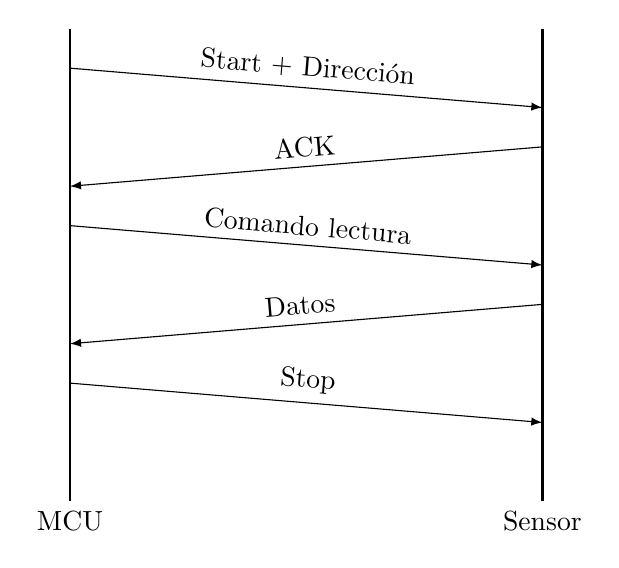
\begin{tikzpicture}[
	node distance=2cm,
	every node/.style={align=center},
	label/.style={draw=none}
	]
	% Líneas de tiempo verticales
	\draw[thick] (0,0) -- (0,-6) node[below] {MCU};
	\draw[thick] (6,0) -- (6,-6) node[below] {Sensor};
	
	% Mensajes
	\draw[-latex] (0,-0.5) -- (6,-1) node[midway, above, sloped] {Start + Dirección};
	\draw[-latex] (6,-1.5) -- (0,-2) node[midway, above, sloped] {ACK};
	\draw[-latex] (0,-2.5) -- (6,-3) node[midway, above, sloped] {Comando lectura};
	\draw[-latex] (6,-3.5) -- (0,-4) node[midway, above, sloped] {Datos \MPF};
	\draw[-latex] (0,-4.5) -- (6,-5) node[midway, above, sloped] {Stop};
	\end{tikzpicture}
	\shorthandon{>}
	\caption{Secuencia de comunicación UART con sensor SPS30.}
	\label{fig:i2c_sequence}
\end{figure}

\subsection{Protocolo SPI para almacenamiento}
Se aplicó el protocolo SPI de comunicación con la memoria microSD. El diseño incorporó las siguientes especificaciones técnicas:

\begin{itemize}
	\item Frecuencia de operación: \SI{42}{\mega\hertz} en modo maestro.
	\item Sistema de archivos: FAT32 con sectores de \SI{512}{\byte}.
	\item Transferencia de datos: DMA para optimización de recursos.
	\item Buffer circular: \SI{512}{\byte} para gestión de escritura.
\end{itemize}

\subsection{UART para comunicación inalámbrica}
La implementación de la comunicación con el módulo ESP8266 estableció una interfaz UART con los siguientes parámetros operativos:
\begin{itemize}
	\item Velocidad de transmisión: \SI{115200}{\baud}.
	\item Control de flujo: señales hardware RTS/CTS.
	\item Buffer de transmisión: \SI{256}{\byte}.
	\item Tiempo de espera máximo: \SI{100}{\milli\second}.
\end{itemize}
La capa de aplicación implementó los siguientes mecanismos de control:
\begin{itemize}
	\item Establecimiento de conexión mediante handshaking.
	\item Sistema de retransmisión automática ante fallos.
	\item Verificación de integridad mediante CRC-16.
	\item Estructura de trama con campos de cabecera y cola.
\end{itemize}

\subsection{GPIO para control y monitoreo}
Se estableció tres funciones principales para la puesta en funcionamiento de las interfaces GPIO :
\begin{itemize}
	\item Señalización visual: control del LED mediante modulación PWM.
	\item Supervisión energética: detección del estado de alimentación.
	\item Control de energía: gestión del modo de bajo consumo.
\end{itemize}
\subsection{Gestión de errores y recuperación}
El sistema implementó mecanismos de protección y recuperación ante fallos de comunicación:
\begin{itemize}
	\item Sistema de temporización: límites de tiempo para cada transacción.
	\item Recuperación automática: reinicialización de periféricos ante errores.
	\item Sistema de respaldo: buffer temporal para datos críticos.
	\item Trazabilidad: registro de eventos de error en memoria no volátil.
\end{itemize}

\subsection{Optimización del rendimiento}
Al instrumento se le incorporó mecanismos específicos para optimizar la eficiencia del sistema:
\begin{itemize}
	\item Transferencia de datos: DMA para operaciones críticas.
	\item Gestión de eventos: sistema de interrupciones para respuesta inmediata.
	\item Administración de memoria: buffers circulares para gestión eficiente.
	\item Planificación: esquema de prioridades para tareas de comunicación.
\end{itemize}

El diseño modular permitió el mantenimiento y actualización independiente de cada protocolo, mientras que los mecanismos de optimización aseguraron un uso eficiente de los recursos del microcontrolador.

	
\section{Ajuste y calibración de sensores y transmisores}
Se estableció un proceso sistemático de calibración y ajuste del sistema de medición de \MPF para asegurar la precisión y trazabilidad de las mediciones. Este procedimiento consideró las características específicas de los sensores SPS30 y las condiciones ambientales de operación.
\subsection{Calibración de sensores \MPF}
El protocolo de calibración se implementó en dos etapas principales:
\begin{enumerate}
	\item Calibración de fábrica: Los sensores incorporaron una calibración inicial contra instrumentos de referencia:
	\begin{itemize}
		\item Fotómetro TSI DustTrak™ DRX 8533: validación gravimétrica.
		\item Espectrómetro óptico TSI OPS 3330: caracterización de distribución de partículas.
	\end{itemize}
	\item Calibración en campo: La implementación requirió ajustes específicos según condiciones locales:

	\begin{itemize}
		\item Correlación con monitor Beta de referencia.
		\item Factor de corrección por humedad relativa.
		\item Compensación por temperatura ambiente.
	\end{itemize}
\end{enumerate}


\subsection{Modelo de corrección}
Se incorporó un modelo de corrección lineal para el ajuste de las mediciones:
\begin{equation}
C_{corregida} = a \cdot C_{medida} + b \cdot H + c \cdot T + d
\end{equation}
Donde las variables representan:
\begin{itemize}
	\item $C_{corregida}$: concentración ajustada (\si{\micro\gram\per\cubic\meter}).
	\item $C_{medida}$: concentración del sensor SPS30.
	\item $H$: humedad relativa (\%).
	\item $T$: temperatura (\si{\celsius}).
	\item $a$, $b$, $c$, $d$: coeficientes determinados  de manera experimental.
\end{itemize}

\subsection{Procedimiento de calibración}
El procedimiento de calibración en campo estableció cinco etapas secuenciales:
\begin{enumerate}
	\item Acondicionamiento inicial: período de estabilización de 24 horas.
	\item Adquisición de datos: mediciones simultáneas con monitor Beta de referencia.
	\item Procesamiento estadístico: determinación de coeficientes mediante regresión lineal.
	\item Verificación: validación con conjunto de datos independiente.
	\item Programación: actualización del firmware con factores de corrección.
\end{enumerate}


\subsection{Validación y control de calidad}
Se ejecutaron mecanismos automáticos para el aseguramiento de la calidad de las mediciones:
\begin{itemize}
	\item Sistema de detección de valores atípicos.
	\item Validación cruzada entre los tres sensores redundantes.
	\item Monitoreo continuo de variables ambientales.
	\item Sistema de notificación para recalibración programada.
\end{itemize}
\subsection{Mantenimiento y recalibración}
El protocolo de mantenimiento estableció un cronograma sistemático de verificación:
\begin{itemize}
	\item Validación trimestral con monitor Beta de referencia.
	\item Ciclo automático de limpieza cada \SI{168}{\hour}.
	\item Recalibración integral anual.
	\item Compensación de la deriva temporal mediante ajuste de coeficientes.
\end{itemize}

Esta implementación sistemática de calibración y control busca asegurar la estabilidad y precisión de las mediciones a largo plazo. La arquitectura con tres sensores permitió la validación continua de datos y la detección temprana de desviaciones en el sistema de medición.

%\section{Análisis del software}
% 
%La idea de esta sección es resaltar los problemas encontrados, los criterios utilizados y la justificación de las decisiones que se hayan tomado.
%
%Se puede agregar código o pseudocódigo dentro de un entorno lstlisting con el siguiente código:
%
%\begin{verbatim}
%\begin{lstlisting}[caption= "un epígrafe descriptivo"]
%	las líneas de código irían aquí...
%\end{lstlisting}
%\end{verbatim}
%
%A modo de ejemplo:
%
%\begin{lstlisting}[label=cod:vControl,caption=Pseudocódigo del lazo principal de control.]  % Start your code-block
%
%#define MAX_SENSOR_NUMBER 3
%#define MAX_ALARM_NUMBER  6
%#define MAX_ACTUATOR_NUMBER 6
%
%uint32_t sensorValue[MAX_SENSOR_NUMBER];		
%FunctionalState alarmControl[MAX_ALARM_NUMBER];	//ENABLE or DISABLE
%state_t alarmState[MAX_ALARM_NUMBER];						//ON or OFF
%state_t actuatorState[MAX_ACTUATOR_NUMBER];			//ON or OFF
%
%void vControl() {
%
%	initGlobalVariables();
%	
%	period = 500 ms;
%		
%	while(1) {
%
%		ticks = xTaskGetTickCount();
%		
%		updateSensors();
%		
%		updateAlarms();
%		
%		controlActuators();
%		
%		vTaskDelayUntil(&ticks, period);
%	}
%}
%\end{lstlisting}



